% !TEX root = task-1-12-1.tex
% Editable task bank. Append new BankTask blocks at the end of the document.
\documentclass[12pt,a4paper]{article}
\usepackage{physics-textbook}
\usepackage{graphicx,needspace}
\usetikzlibrary{decorations.pathmorphing}
\newif\ifShowSolutions
\ifdefined\TutorEdition
  \ShowSolutionstrue
\else
  \ShowSolutionsfalse % Change to \ShowSolutionstrue to display solutions.
\fi
\newcounter{banktask}
\newsavebox{\BankTaskBox}
\newcommand{\BankTaskContent}[3]{%
  \noindent\textbf{\thebanktask.}\quad #2\par
  \ifShowSolutions
    \Needspace{50mm}% Keep the solution heading with its opening text or diagram.
    #3\par
    \ifdefined\TutorEdition
      \ifcsname TutorSource#1\endcsname
        \nopagebreak\smallskip{\small\csname TutorSource#1\endcsname\par}%
      \fi
    \fi
  \fi
}
\newcommand{\BankTask}[3]{%
  \refstepcounter{banktask}\par\medskip
  \sbox{\BankTaskBox}{\begin{minipage}{\linewidth}%
    \BankTaskContent{#1}{#2}{#3}\end{minipage}}%
  \ifdim\dimexpr\ht\BankTaskBox+\dp\BankTaskBox\relax>\dimexpr\textheight-20mm\relax
    \Needspace{35mm}\BankTaskContent{#1}{#2}{#3}%
  \else
    \Needspace{\dimexpr\ht\BankTaskBox+\dp\BankTaskBox\relax}%
    \noindent\usebox{\BankTaskBox}\par
  \fi
  \medskip
}
\begin{document}
\BookSubsection{1.12.1}{Момент силы}


% Source sdamgia-26715: https://phys-ege.sdamgia.ru/problem?id=26715
\BankTask{sdamgia-26715}{
На рычаг действуют две силы. Момент первой силы относительно оси вращения рычага равен $50\,\text{Н}\cdot\text{м}$. Какова величина второй силы, если ее плечо относительно этой же оси равно $0{,}5 \,\text{м}$ и рычаг при этом находится в равновесии?
}{
\smallskip\noindent\textbf{Решение}\par
Так как рычаг находится в равновесии, то по правилу моментов $M_{1}=M_{2} .$ Момент второй силы равен $M_{2} =F_{2} \cdot d_{2} .$ Откуда находим величину второй силы:

$F_{2} = \frac{ M_{2} }{ d_{2} } = \frac{ 50\,\text{Н} \cdot \,\text{м}}{ 0{,}5\,\text{м} } =100\,\text{Н}.$

Ответ: $100$.
}

% Source sdamgia-50713: https://phys-ege.sdamgia.ru/problem?id=50713
\BankTask{sdamgia-50713}{
Невесомый рычаг находится в равновесии. Левое плечо рычага равно $6 \,\text{см}$, правое плечо равно $15 \,\text{см}$. На правом плече подвешен груз массой $0{,}2 \,\text{кг}$. Какой массы груз нужно подвесить на левом плече, чтобы рычаг оставался в равновесии?
}{
\smallskip\noindent\textbf{Решение}\par
По правилу моментов $m_{1}g l_{1}=m_{2}g l_{2},$ откуда масса груза на левом плече равна

$m_{1}= \frac{ m_{2}l_{2}}{ l_{1} } = \frac{ 0{,}2 \cdot 15}{ 6 } =0{,}5\,\text{кг}.$

Ответ: $0{,}5$.
}

% Source sdamgia-38513: https://phys-ege.sdamgia.ru/problem?id=38513
\BankTask{sdamgia-38513}{
Ученик выполнял лабораторную работу по исследованию условий равновесия лёгкого рычага, к которому приложены силы $F_{1}$ и $F_{2}$. Результаты, которые он получил, представлены в таблице. $l_{1}$, $l_{2}$ — плечи сил. Каков модуль силы $F_{2}$, если рычаг находится в равновесии?

\begin{center}\begin{tabular}{|c|c|c|c|}\hline
$F_{1}$, Н&$l_{1}$, м&$F_{2}$, Н&$l_{2}$, м\\\hline
$40$&$1{,}2$&$?$&$0{,}8$\\\hline
\end{tabular}\end{center}
}{
\smallskip\noindent\textbf{Решение}\par
Рычаг находится в равновесии, если выполняется правило моментов приложенных сил: $F_{1}l_{1}=F_{2}l_{2},$ откуда находим вторую силу:

$F_{2} = \frac{ F_{1}l_{1}}{ l_{2} } = \frac{ 40 \cdot 1{,}2}{ 0{,}8 } = 60 \,\text{Н}.$

Ответ: $60$.
}

% Source sdamgia-35923: https://phys-ege.sdamgia.ru/problem?id=35923
\BankTask{sdamgia-35923}{
\begin{center}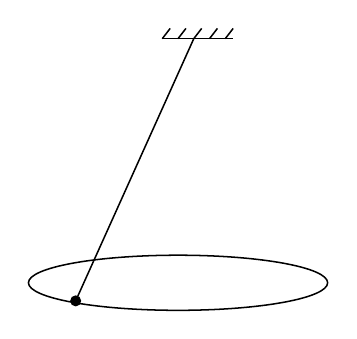
\begin{tikzpicture}[x=1cm,y=1cm,>=stealth,line width=.55pt]
\draw (0,0) ellipse (1.9 and .35);\draw (.2,3.1)--(-1.3,-.23);\draw (-.2,3.1)--(.7,3.1);\foreach \x in {-.2,0,...,.7}{\draw (\x,3.1)--++(.1,.13);}\fill (-1.3,-.23) circle(2pt);
\end{tikzpicture}\end{center}
Грузик массой $0{,}2 \,\text{кг}$ привязан к нити длиной $1 \,\text{м}$ и вращается в горизонтальной плоскости по окружности радиусом $0{,}3 \,\text{м}$. Чему равен момент силы тяжести относительно горизонтальной оси, проходящей через точку подвеса перпендикулярно плоскости рисунка?
}{
\smallskip\noindent\textbf{Решение}\par
Плечо силы тяжести $F_{\text{тяж}}=mg$ равно радиусу окружности. Тогда момент данной силы равен:

$M = mgR=0{,}2 \cdot 10 \cdot 0{,}3=0{,}6 \,\text{Н} \cdot \,\text{м} .$

Ответ: $0{,}6$.
}

% Source sdamgia-38044: https://phys-ege.sdamgia.ru/problem?id=38044
\BankTask{sdamgia-38044}{
\begin{center}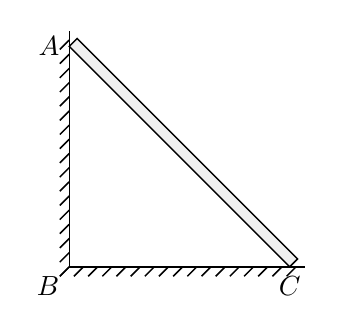
\begin{tikzpicture}[x=1cm,y=1cm,>=stealth,line width=.55pt]
\draw (0,0)--(0,3);\foreach \y in {0,0.18,...,3}{\draw (0,\y)--++(-.12,-.12);}\draw (0,0)--(3,0);\foreach \x in {0,0.18,...,3}{\draw (\x,0)--++(-.12,-.12);}\draw[fill=gray!12] (0,2.8)--(.1,2.9)--(2.9,.1)--(2.8,0)--cycle;\node[left] at (0,2.8){$A$};\node[below left] at (0,0){$B$};\node[below] at (2.8,0){$C$};
\end{tikzpicture}\end{center}
На рисунке изображена прямая однородная доска АС, прислонённая к вертикальной стене AB. Чему равен момент силы тяжести, действующей на эту доску, относительно оси, проходящей через точку В перпендикулярно плоскости рисунка? Масса доски равна $12 \,\text{кг}$, расстояние от прямого угла В до нижнего конца доски равно $BC=1{,}2\,\text{м}$.
}{
\smallskip\noindent\textbf{Решение}\par
\begin{center}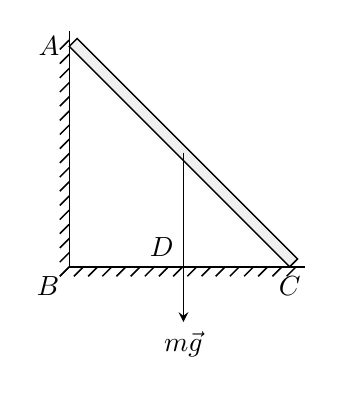
\begin{tikzpicture}[x=1cm,y=1cm,>=stealth,line width=.55pt]
\draw (0,0)--(0,3);\foreach \y in {0,0.18,...,3}{\draw (0,\y)--++(-.12,-.12);}\draw (0,0)--(3,0);\foreach \x in {0,0.18,...,3}{\draw (\x,0)--++(-.12,-.12);}\draw[fill=gray!12] (0,2.8)--(.1,2.9)--(2.9,.1)--(2.8,0)--cycle;\node[left] at (0,2.8){$A$};\node[below left] at (0,0){$B$};\node[below] at (2.8,0){$C$};\draw[->] (1.45,1.45)--(1.45,-.7) node[below]{$m\vec g$};\node[above left] at (1.45,0){$D$};
\end{tikzpicture}\end{center}

Момент силы тяжести равен $M=mg \cdot BD.$ Так как доска однородная, то сила тяжести приложена к её середине. Из соотношения сторон прямоугольного треугольника получаем, что $BD= \frac{ 1}{ 2 } BC.$
Таким образом, момент силы тяжести относительно оси, проходящей через точку В равен

$M = \frac{ mg \cdot BC}{ 2 } = \frac{ 12 \cdot 10 \cdot 1{,}2}{ 2 } =72 \,\text{Н} \cdot \,\text{м} .$

Ответ: $72$.
}

% Source sdamgia-27082: https://phys-ege.sdamgia.ru/problem?id=27082
\BankTask{sdamgia-27082}{
Тяжелая однородная рейка может вращаться вокруг горизонтальной оси, проходящей через точку О (см. рис.).

\begin{center}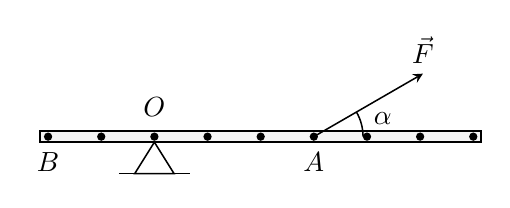
\begin{tikzpicture}[x=1cm,y=1cm,>=stealth,line width=.55pt]
\draw[fill=gray!8] (0,0) rectangle (5.6,.14);\foreach \i in {0,...,8}{\fill (.1+.675*\i,.07) circle(1.5pt);}\draw (1.45,0)--(1.2,-.4)--(1.7,-.4)--cycle;\draw (1,-.4)--(1.9,-.4);\node[above] at (1.45,.2){$O$};\node[below] at (.1,0){$B$};\node[below] at (3.475,0){$A$};\draw[->] (3.475,.07)--++(30:1.6) node[above]{$\vec F$};\draw (4.1,.07) arc(0:30:.625);\node at (4.35,.3){$\alpha$};
\end{tikzpicture}\end{center}

В рейке проделаны небольшие отверстия (они показаны на рисунке черными точками). Расстояние между соседними отверстиями $8 \,\text{см}$. С помощью силы $F=10 \,\text{Н}$, приложенной в точке А и направленной под углом $\alpha =30 ^\circ$ к рейке, она удерживается в равновесии. Чему равен модуль момента силы $F$ относительно горизонтальной оси, проходящей через точку $B$?
}{
\smallskip\noindent\textbf{Решение}\par
Плечо силы $F$ относительно точки В равно $d=5 \cdot 0{,}08 \cdot \sin 30 ^\circ =0{,}2\,\text{м}.$ Тогда момент силы относительно точки В найдем по формуле $M=F \cdot d=10\,\text{Н} \cdot 0{,}2\,\text{м}=2\,\text{Н} \cdot \,\text{м}.$
 
Ответ: $2$.
}

% Source sdamgia-9731: https://phys-ege.sdamgia.ru/problem?id=9731
\BankTask{sdamgia-9731}{
\begin{center}\begin{tikzpicture}[x=1cm,y=1cm,>=stealth,line width=.55pt]
\draw (0,0) circle(1);\draw (0,0) circle(.43);\fill (0,0) circle(1.5pt);\draw (0,0)--(0,1.8);\draw (-.9,1.8)--(.9,1.8);\foreach \x in {-.9,-.7,...,.9}{\draw (\x,1.8)--++(.12,.12);}\draw (-.43,0)--(-.43,-1.8);\draw (1,0)--(1,-1.35);\draw[fill=gray!15] (-.63,-2.3) rectangle (-.23,-1.8);\draw[fill=gray!15] (.8,-1.85) rectangle (1.2,-1.35);\node[below] at (-.43,-2.3){$8\,\text{кг}$};\node[below] at (1,-1.85){$2\,\text{кг}$};
\end{tikzpicture}\end{center}
Ступенчатый блок имеет внутренний шкив радиусом $6 \,\text{см}$. К нитям, намотанным на внешний и внутренний шкивы, подвешены грузы так, как показано на рисунке. Трение в оси блока отсутствует. Чему равен радиус внешнего шкива блока, если система находится в равновесии?
}{
\smallskip\noindent\textbf{Решение}\par
Так как блок находится в равновесии, то моменты сил, действующих на него должны быть равны:

$m_{1}l_{1}=m_{2}l_{2}.$

Найдем отсюда радиус внешнего шкива:

$l_{2}= \frac{ m_{1}l_{1}}{ m_{2} } = \frac{ 8 \cdot 6}{ 2 } =24\,\text{см}.$

Ответ: $24$.
}

% Source sdamgia-26733: https://phys-ege.sdamgia.ru/problem?id=26733
\BankTask{sdamgia-26733}{
\begin{center}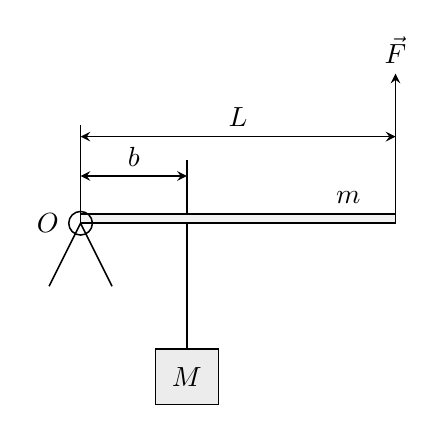
\begin{tikzpicture}[x=1cm,y=1cm,>=stealth,line width=.55pt]
\draw[fill=gray!10] (0,0) rectangle (4,.12);\draw (0,0) circle (.15);\draw (-.4,-.8)--(0,0)--(.4,-.8);\draw[<->] (0,1.1)--(4,1.1) node[midway,above]{$L$};\draw (0,.12)--(0,1.25);\draw (4,.12)--(4,1.4);\draw[<->] (0,.6)--(1.35,.6) node[midway,above]{$b$};\draw (1.35,.12)--(1.35,.8);\draw[->] (4,0)--(4,1.9) node[above]{$\vec F$};\node[left] at (-.15,0){$O$};\node[above] at (3.4,.12){$m$};\draw (1.35,0)--(1.35,-1.6);\draw[fill=gray!15] (.95,-2.3) rectangle (1.75,-1.6);\node at (1.35,-1.95){$M$};
\end{tikzpicture}\end{center}
Груз массой $M=75 \,\text{кг}$ медленно поднимают с помощью рычага, приложив вертикальную силу $\vec{F}$ (см. рис.). Рычаг, сделанный из однородного стержня массой $m=10 \,\text{кг}$ и длиной $L=4 \,\text{м}$, шарнирно закреплен. Определите модуль силы $\vec{F},$ если расстояние $b$ от оси шарнира до точки подвеса груза равно $1{,}6 \,\text{м}$. Считать, что трение в шарнире отсутствует.
}{
\smallskip\noindent\textbf{Решение}\par
\begin{center}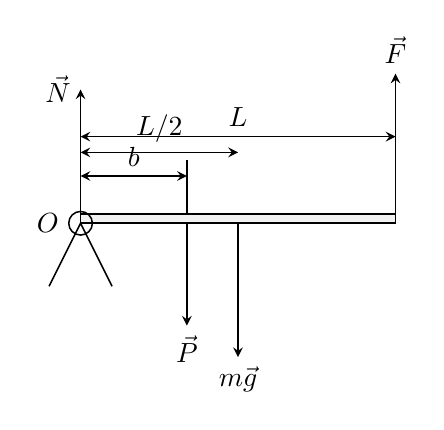
\begin{tikzpicture}[x=1cm,y=1cm,>=stealth,line width=.55pt]
\draw[fill=gray!10] (0,0) rectangle (4,.12);\draw (0,0) circle (.15);\draw (-.4,-.8)--(0,0)--(.4,-.8);\draw[<->] (0,1.1)--(4,1.1) node[midway,above]{$L$};\draw (0,.12)--(0,1.25);\draw (4,.12)--(4,1.4);\draw[<->] (0,.6)--(1.35,.6) node[midway,above]{$b$};\draw (1.35,.12)--(1.35,.8);\draw[->] (4,0)--(4,1.9) node[above]{$\vec F$};\node[left] at (-.15,0){$O$};\draw[->] (1.35,0)--(1.35,-1.3) node[below]{$\vec P$};\draw[->] (2,0)--(2,-1.7) node[below]{$m\vec g$};\draw[->] (0,0)--(0,1.7) node[left]{$\vec N$};\draw[<->] (0,.9)--(2,.9) node[midway,above]{$L/2$};
\end{tikzpicture}\end{center}

\par\smallskip\noindent $1$. Рассмотрим силы, действующие на рычаг (см. рис.). 
Считая, что рычаг поднимает груз медленно и равномерно, примем, исходя из третьего и второго законов Ньютона, что $|\vec{P} |=|M \vec{g}|.$
\par\smallskip\noindent $2$. Рассмотрим равновесие рычага относительно оси вращения — шарнира О, указав плечи сил на рисунке. $O: Mg \cdot b + \frac{ 1}{ 2 } mgL - FL=0.$
Отсюда:

$F=Mg \cdot \frac{ b}{ L } + \frac{ 1}{ 2 } mg=75 \cdot 10 \cdot \frac{ 1{,}6}{ 4 } + \frac{ 1}{ 2 } \cdot 10 \cdot 10=350\,\text{Н}.$

 
Ответ: $F=350 \,\text{Н}$.
}

% Source sdamgia-25401: https://phys-ege.sdamgia.ru/problem?id=25401
\BankTask{sdamgia-25401}{
Деревянная линейка длиной $l=90 \,\text{см}$ выдвинута за край стола на $\frac{ 1}{ 4 }$ часть своей длины. При этом она не опрокидывается, если на ее правом конце лежит груз массой не более $m_{1}=250\,\text{г}.$ Далее линейку выдвинули вправо за край стола на некоторое расстояние и положили на ее правый конец груз массой $m_{2}=125\,\text{г}.$ На какое расстояние дополнительно можно выдвинуть линейку во втором опыте, чтобы она не перевернулась?
}{
\smallskip\noindent\textbf{Решение}\par
На линейку в обоих случаях действую сила тяжести линейки, приложенная к ее середине и вес груза. Линейка находится в равновесии, поэтому можно записать правило моментов для каждого случая относительно точки опоры — края стола. В первом случае плечи силы тяжести линейки и веса груза равны $\frac{ l}{ 4 } .$ 
Следовательно, масса линейки равна массе груза $M=m_{1}=250\,\text{г}.$

\begin{center}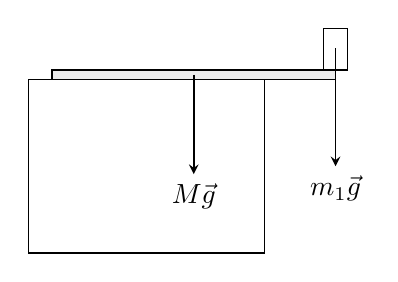
\begin{tikzpicture}[x=1cm,y=1cm,>=stealth,line width=.55pt]
\draw (0,-2.2) rectangle (3,0);\draw[fill=gray!15] (0.3,0) rectangle (3.9,.12);\draw[fill=white] (3.75,.12) rectangle (4.05,.65);\draw[->] (2.1,.06)--(2.1,-1.2) node[below]{$M\vec g$};\draw[->] (3.9,.4)--(3.9,-1.1) node[below]{$m_1\vec g$};
\end{tikzpicture}\end{center}

\begin{center}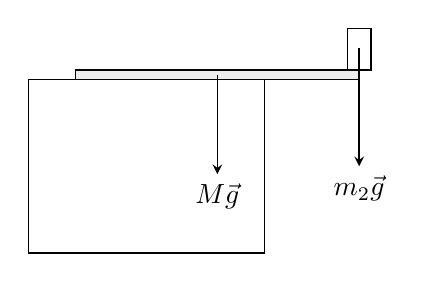
\begin{tikzpicture}[x=1cm,y=1cm,>=stealth,line width=.55pt]
\draw (0,-2.2) rectangle (3,0);\draw[fill=gray!15] (0.6,0) rectangle (4.2,.12);\draw[fill=white] (4.05,.12) rectangle (4.3500000000000005,.65);\draw[->] (2.4,.06)--(2.4,-1.2) node[below]{$M\vec g$};\draw[->] (4.2,.4)--(4.2,-1.1) node[below]{$m_2\vec g$};
\end{tikzpicture}\end{center}

Во втором случае плечо веса груза равно $l_{2}$ а плечо силы тяжести линейки $\frac{ l}{ 2 } - l_{2}.$
Запишем правило моментов для второго случая:

$m_{2}gl_{2}=Mg ( \frac{ l}{ 2 } - l_{2} ) ,$ откуда плечо веса груза:
$l_{2}= \frac{ Ml}{ 2 ( m_{2} + M ) } = \frac{ 250 \cdot 90}{ 2 \cdot ( 125 + 250 ) } =30\,\text{см}.$

Учитывая, что в первом случае расстояние равнялось $\frac{ l}{ 4 } = \frac{ 90}{ 4 } =22{,}5\,\text{см},$ линейка останется в равновесии, если ее выдвинуть на $7{,}5 \,\text{см}$.
 
Ответ: $7{,}5 \,\text{см}$.
}

% Source sdamgia-3418: https://phys-ege.sdamgia.ru/problem?id=3418
\BankTask{sdamgia-3418}{
Однородную балку поднимают за один конец, прикладывая силу $\vec{F}$ перпендикулярно балке. На рисунке показан график изменения модуля силы по мере подъема конца балки. 

 

\begin{center}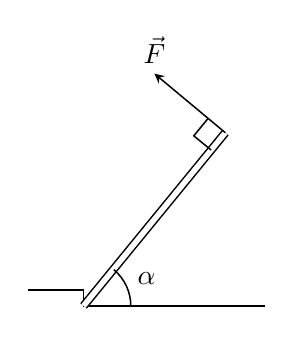
\begin{tikzpicture}[x=1cm,y=1cm,>=stealth,line width=.55pt]
\draw (-.7,0)--(0,0)--(0,-.2)--(2.3,-.2);\draw[double,double distance=2pt] (0,-.2)--(1.8,2);\draw[->] (1.8,2)--(.9,2.75) node[above]{$\vec F$};\draw (1.62,1.78)--(1.4,1.96)--(1.58,2.18);\draw (.6,-.2) arc(0:50:.6);\node at (.8,.15){$\alpha$};
\end{tikzpicture}\end{center}

\begin{center}\begin{tikzpicture}[x=1cm,y=1cm,>=stealth,line width=.55pt]
\draw[step=.5,gray!50,thin] (0,0) grid (3,3);\draw[->] (-.25,0)--(3.4,0) node[right]{$\alpha,\ \text{рад}$};\draw[->] (0,-.25)--(0,3.35) node[above]{$F,\ \text{Н}$};\draw[thick] (0,2) arc(90:0:2);\foreach \y/\v in {.5/100,1/200,1.5/300,2/400}{\node[left] at(0,\y){$\v$};}\node[below left] at(0,0){$0$};\node[below] at(2,0){$\pi/2$};
\end{tikzpicture}\end{center}

Чему равна масса балки?
}{
\smallskip\noindent\textbf{Решение}\par
Проще всего определить массу балки, рассмотрев самое начало подъема. Для того чтобы правый конец балки начал подниматься, вращающий момент, создаваемый силой $\vec{F}$ относительно левого конца балки, должен стать больше момента, создаваемого силой тяжести относительно этой точки. Сила тяжести приложена к центру масс балки. Поскольку балка однородная, ее центр масс расположен посередине. Обозначим длину балки через $L.$ По правилу моментов приложенных сил $Mg \frac{ L}{ 2 } =FL.$ 
Следовательно, масса балки равна $M= \frac{ 2F}{ g } .$ Из графика видно, что в самом начале для подъема балки была необходима сила в $400 \,\text{Н}$. Следовательно, масса балки равна $M=\frac{2\cdot400}{10}=80\,\text{кг}$.
 
Ответ: $80 \,\text{кг}$.
}


% Source 42654: https://phys-ege.sdamgia.ru/problem?id=42654
\BankTask{42654}{
\begin{center}\begin{tikzpicture}[task graph,>=stealth]
\draw(-.3,0)--(3,0)--(3,-.8);
\foreach \x in {0,.2,...,2.8}{\draw(\x,0)--++(-.12,-.12);}
\draw[fill=white](0,0)rectangle(4,.18);
\node[above left]at(0,.18){$A$};\node[right]at(4,.18){$B$};\node[above]at(2,.18){$M$};
\draw(4,.18)--(4,2.5);\draw(4.6,2.5)circle(.6)(4.6,2.5)circle(1.2);
\draw(5.8,2.5)--(5.8,-.4);\draw[fill=white](5.5,-1)rectangle(6.1,-.4);\node at(5.8,-.7){$m$};
\draw[fill=white](4.23,4)--(4.52,2.48)--(4.68,2.48)--(4.97,4)--cycle;\node at(4.6,2.64){$\times$};\draw(3.55,4)--(5.65,4);
\foreach \x in {3.6,3.8,...,5.6}{\draw(\x,4)--++(.12,.12);}
\node[left]at(3.4,2.5){$R$};\node at(4.65,2.1){$r$};
\end{tikzpicture}\end{center}Однородный брусок $AB$ массой $M$ постоянного прямоугольного сечения лежит на гладкой горизонтальной поверхности стола, свешиваясь с него менее чем наполовину (см. рисунок). К правому концу бруска прикреплена легкая нерастяжимая нить. Другой конец нити закреплен на меньшем из двух дисков идеального составного блока. На большем диске этого блока закреплена другая легкая нерастяжимая нить, на которой висит груз массой $m$. Диски скреплены друг с другом, образуя единое целое, где $R$  =  $10\,\text{см}$, $r$  =  $5\,\text{см}$.
Сделайте рисунок с указанием сил, действующих на брусок $M$, блок и груз $m$. Найдите максимальное значение дроби  $\frac{m}{M} ,$ при котором система тел остается неподвижной. Трением в оси блока пренебречь. Обоснуйте применимость используемых законов к решению задачи.
}{
\smallskip\noindent\textbf{Решение}\par
Обоснование. 
$1$.  Систему отсчета, связанную с Землей, будем считать инерциальной (ИСО). 
$2$.  Брусок перед отрывом его правого края от поверхности стола будем считать твердым телом с осью вращения, проходящей перпендикулярно плоскости рисунка через точку $A$. Условие равновесия относительно вращения твердого тела на оси  — равенство нулю суммы моментов сил, приложенных к телу, относительно этой оси. 
$3$.  Нити нерастяжимы, поэтому, если покоится брусок, то покоятся и все остальные тела системы. $4$. Нити легкие, поэтому величина силы натяжения каждой нити в любой ее точке одна и та же. В том числе: $T_1=T_3,$ $T_2=T_4$ (см. рис. в решении). 
$5$.  Блок идеальный (трения в осях нет, масса блока пренебрежимо мала). Поэтому условие равновесия блока  — равенство нулю суммы моментов сил натяжения нитей относительно оси блока. 
$6$.  Груз может двигаться только поступательно вдоль вертикальной оси $Oy$, лежащей в плоскости рисунка. Поэтому для груза используем модель материальной точки и применим второй закон Ньютона. Вследствие этого условие равновесия - сумма приложенных к грузу сил равна нулю.
Решение.\begin{center}\begin{tikzpicture}[task graph,>=stealth]\draw(-.3,0)--(3,0)--(3,-.7);\draw[very thick](0,.08)--(3.8,.08);\node[above left]at(0,.08){$A$};\node[right]at(3.8,.08){$B$};\draw(3.8,.08)--(3.8,2);\draw(4.3,2)circle(.5)(4.3,2)circle(.8);\draw(5.1,2)--(5.1,-.6);\draw[fill=gray!15](4.9,-.9)rectangle(5.3,-.5);\draw[fill=white](4.07,3.2)--(4.22,1.94)--(4.38,1.94)--(4.53,3.2)--cycle;\draw(3.45,3.2)--(5.15,3.2);\draw[->](-.4,0)--(6,0)node[right]{$x$};\draw[->](.7,-1.2)--(.7,1.6)node[above]{$y$};\node[below left]at(.7,0){$O$};\draw[->,thick](0,.08)--(0,.9)node[above left]{$\vec N$};\draw[->,thick](1.9,.08)--(1.9,-1.1)node[right]{$M\vec g$};\draw[->,thick](3.8,.08)--(3.8,.85)node[left]{$\vec T_1$};\draw[->,thick](3.8,2)--(3.8,1.35)node[left]{$\vec T_3$};\draw[->,thick](5.1,2)--(5.1,1.15)node[right]{$\vec T_4$};\draw[->,thick](4.3,2)--(4.3,3.6)node[above]{$\vec F$};\draw[->,thick](5.1,-.5)--(5.1,.35)node[right]{$\vec T_2$};\draw[->,thick](5.1,-.9)--(5.1,-1.6)node[right]{$m\vec g$};\end{tikzpicture}\end{center}
$1$.  Силы, действующие на брусок, блок и груз, показаны на рисунке для случая, когда масса бруска минимальна, и поэтому он еще покоится на столе, но касается стола только в точке $A$. Поэтому сила $\vec N$ приложена к бруску в точке $A$ и направлена вертикально вверх, так как поверхность стола гладкая (трения нет). 
$2$.  Запишем уравнение моментов сил для бруска в момент, когда он покоится, касаясь стола только в точке $A$: 

\[T_1 \cdot A B - M g \cdot \frac{A B}{2} =0,\]

 откуда 

\[T_1= \frac{M g}{2} .\]

$3$.  Запишем второй закон Ньютона для покоящегося груза в проекциях на ось Оу введенной ИСО: $T_2 - m g=0,$ откуда $T_2=m g.$ 
$4$.  Условие равновесия блока на его оси: $T_3 \cdot r=T_4 \cdot R .$ С учетом того, что $T_1=T_3$ и $T_2=T_4,$ получим отсюда $T_1 \cdot r=T_2 \cdot R .$
$5$.  Подставив в это равенство результаты п. $2$ и $3$, получим: 

\[\frac{M g}{2} \cdot r=m g \cdot R.\]

Искомое отношение будет максимальным, если масса $M$ будет минимальной. Найдем это отношение:

\[\frac{m}{M} = \frac{r}{2R} = \frac{5}{2 \cdot 10} =0{,}25.\]

Ответ: $0{,}25$.
}

\end{document}
